\textbf{Golang}

Uno de los puntos centrales de este trabajo es exponer el estado del arte en el uso de Golang para el desarrollo de software que enfrente problemas de tiempo real y interacción con hardware para control automático de actuadores. En dicho estudio se ha consultado distintos papers y publicaciones para extraer primeras conclusiones.

Los recursos consumidos por el lenguaje es uno de los primeros puntos que se deben evaluar. Cual es el coste de hardware para ejecutar el código. La interacción del lenguaje con la base de datos, en concreto mysql por ser la más extendida, es uno de los primeros puntos que se ponen a prueba. En una comparación con Node.js, un framework muy extendido de javascript, la conclusión que extrae el estudio es la siguiente: “\ldots combination of Go and MySQL is superior regarding CPU utilization and memory usage, while Node.js and MySQL combination is superior regarding response time~\cite{Effendy20211955}“. No es relevantemente inferior ni superior.

Otra aplicación del lenguaje que pone a pureba la utilización de RAM y CPU son los algorítmos intensivos. En algorítmia con altos requerimientos, en particular la implementacion de un árbol de decisiones~\cite{Dymora20201} se extra la siguiente conclusión: golang vuelve a no dar ventajas, tampoco inconvenientes, en materia de tiempos de ejecución. Teniendo peor rendimiento en uso de cpu significativamente y empata en materia de uso de memoria para mas de 500K registros en este problema en particular. Aunque se admite que no se ha explotado toda la optimización que el lenguaje permite para este tipo de problemas en particular “Thus, the Go language garbage collector supports programmers by automatically releasing their programs memory when it is no longer needed. However, tracking and cleaning the memory requires additional resources such as CPU time. The effect of this can be seen in Figure 5. Of course, the scope of optimizing“~\cite{Dymora20201}. Quiere decir que una de las ventajas que ofrece golang es no ocuparse del Garbage collector, que si bien ofrece muchas garantías con respecto a otros lenguajes de cara a no sufrir leaks de memoria puede ser un inconveniente en ejecuciones de este tipo y por tanto requerir optimización. El garbage collector le requiere un uso adicional de memoria y cpu para ejecuciones con un gran número de registros. Concluye este estudio diciendo: “. Go can be an attractive alternative in the area of DevOps tools. It is attractive to build something small–medium that works natively without using a lot of RAM and which runs fast with many things needed for this task in the language itself“ ~\cite{Dymora20201}. La conclusión final a este respecto es que si bien para usos intensivos golang es una opción viable no da ventaja. Es en la implementación de algoritmos que sacan ventaja de la concurrencia donde golang puede sacar ventaja respecto a otros lenguages como java o python ~\cite{Jenkins201714}

\begin{figure}[H]
	\centering
	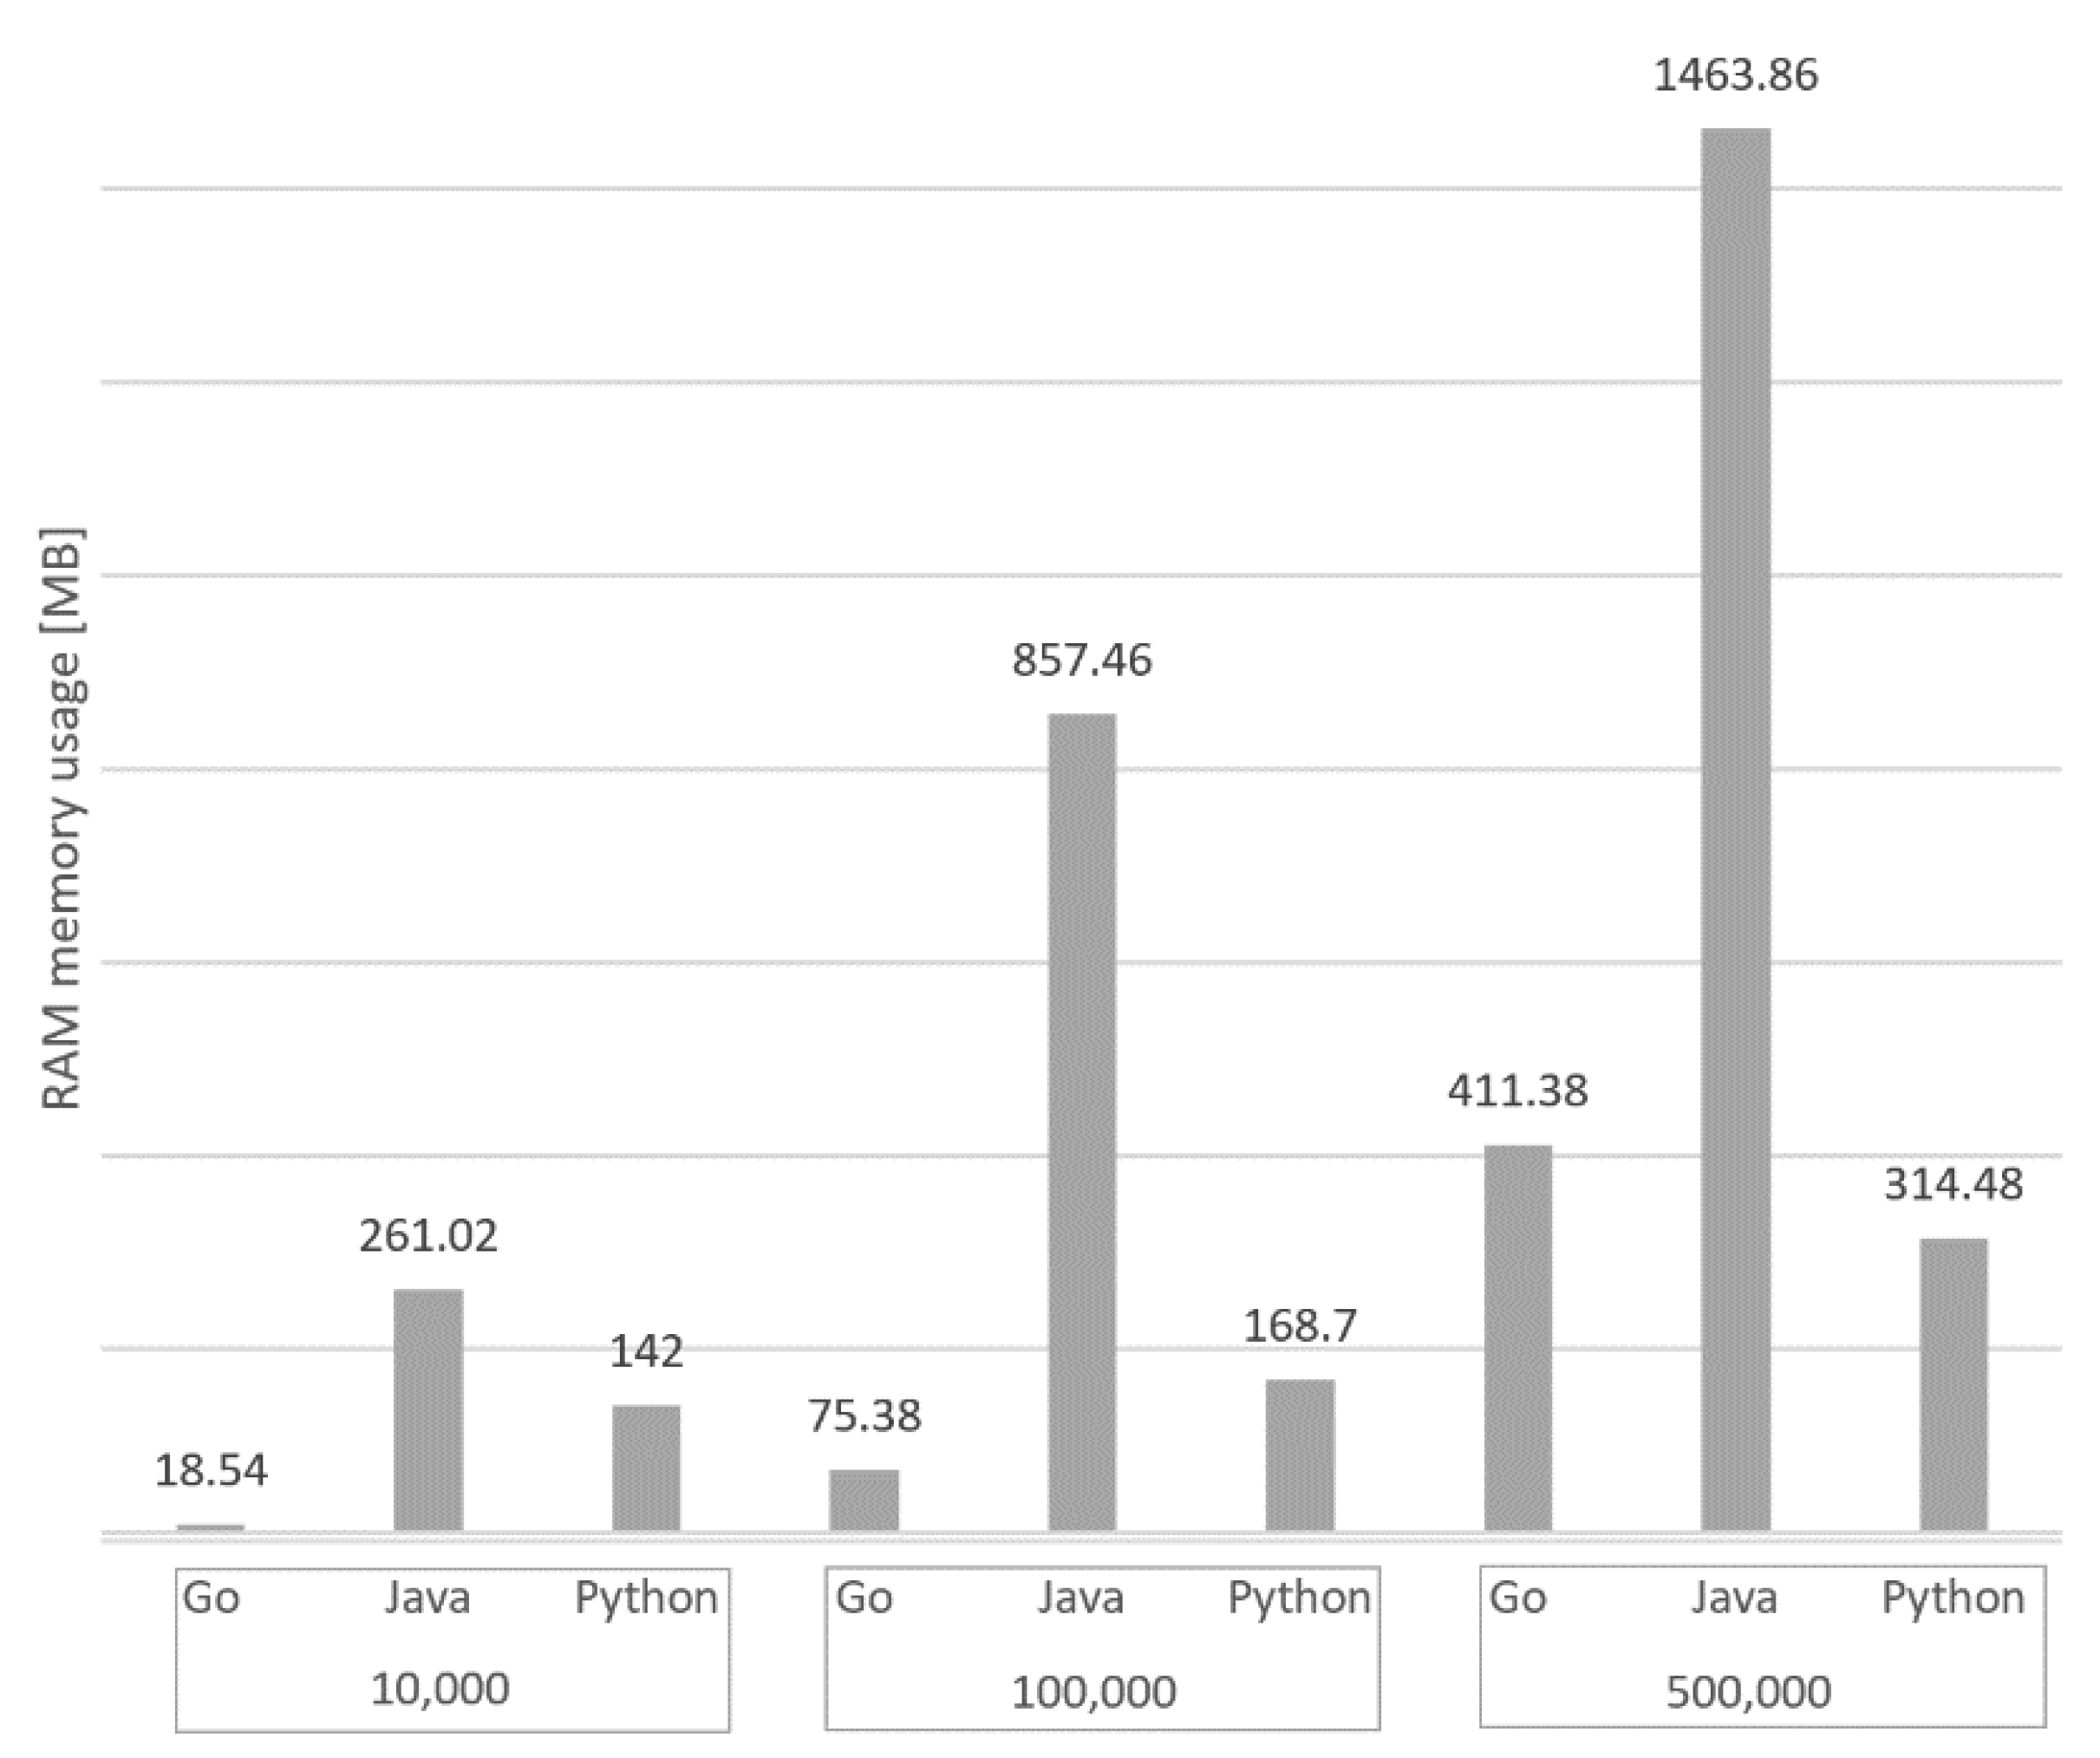
\includegraphics[height=0.3\textheight]{./part/Proyecto_ejecutivo/memoria_constructiva/golang/img/memory_usage}
	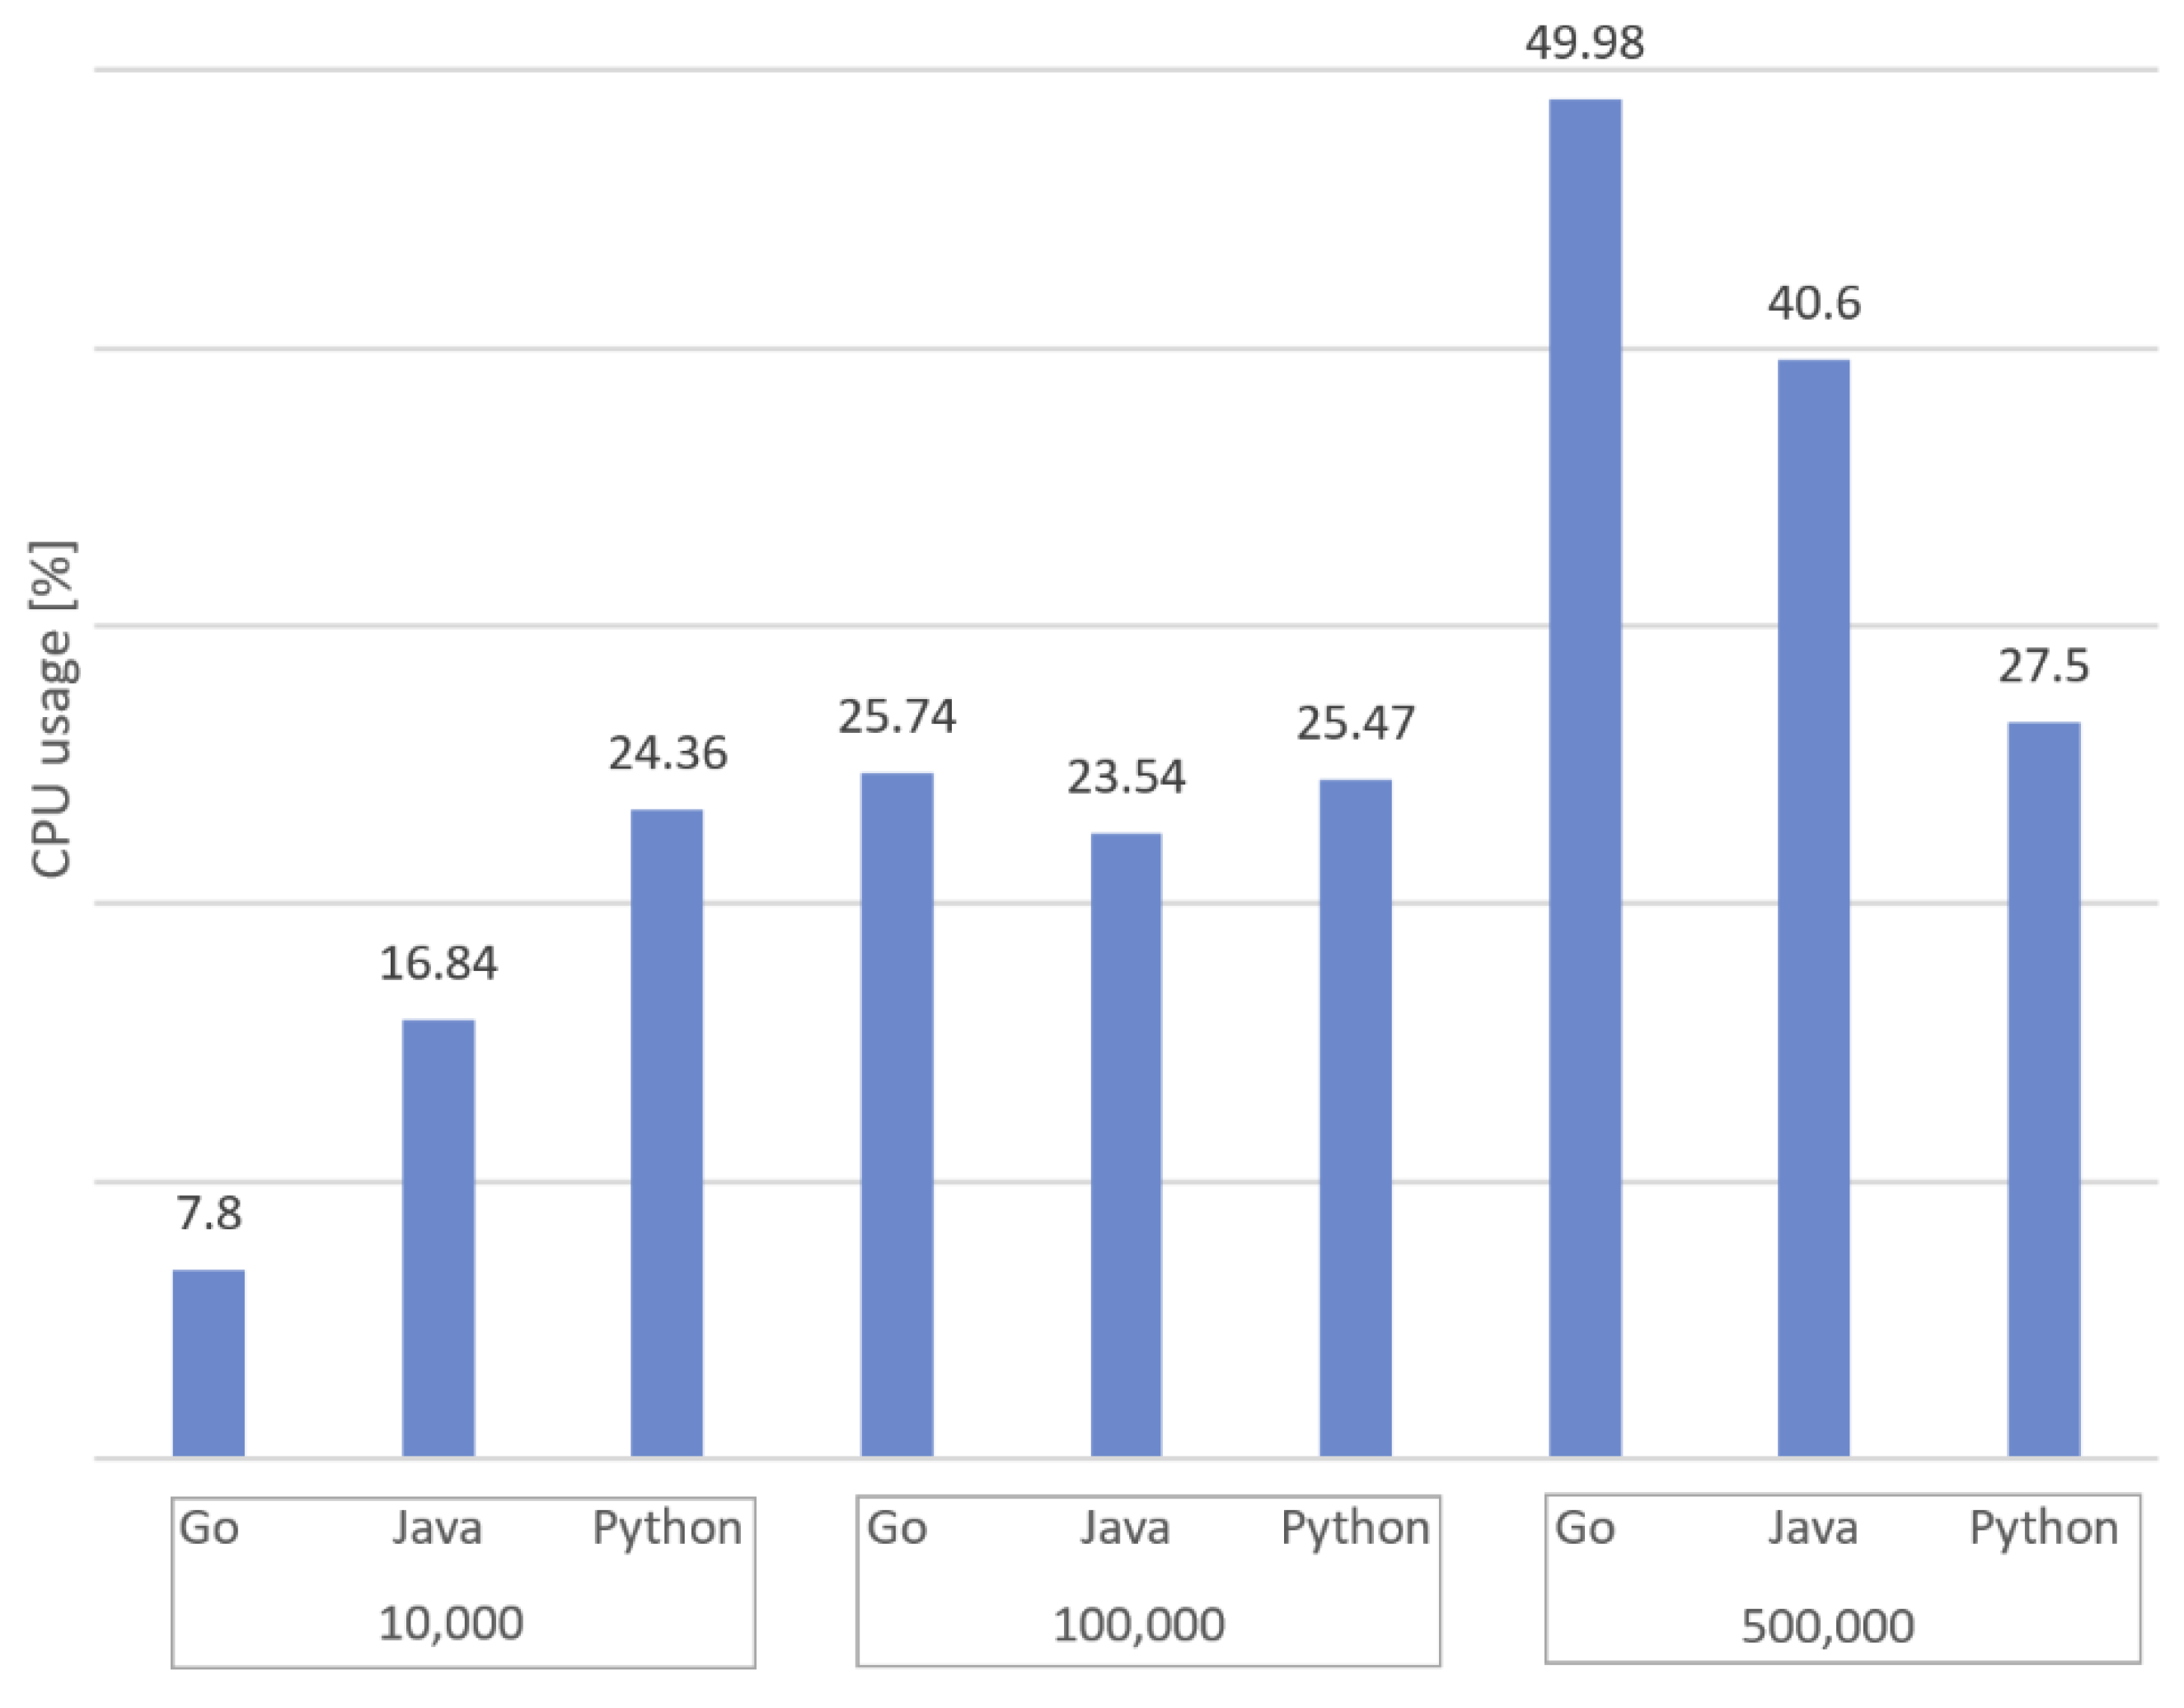
\includegraphics[height=0.3\textheight]{./part/Proyecto_ejecutivo/memoria_constructiva/golang/img/cpuUsage}
	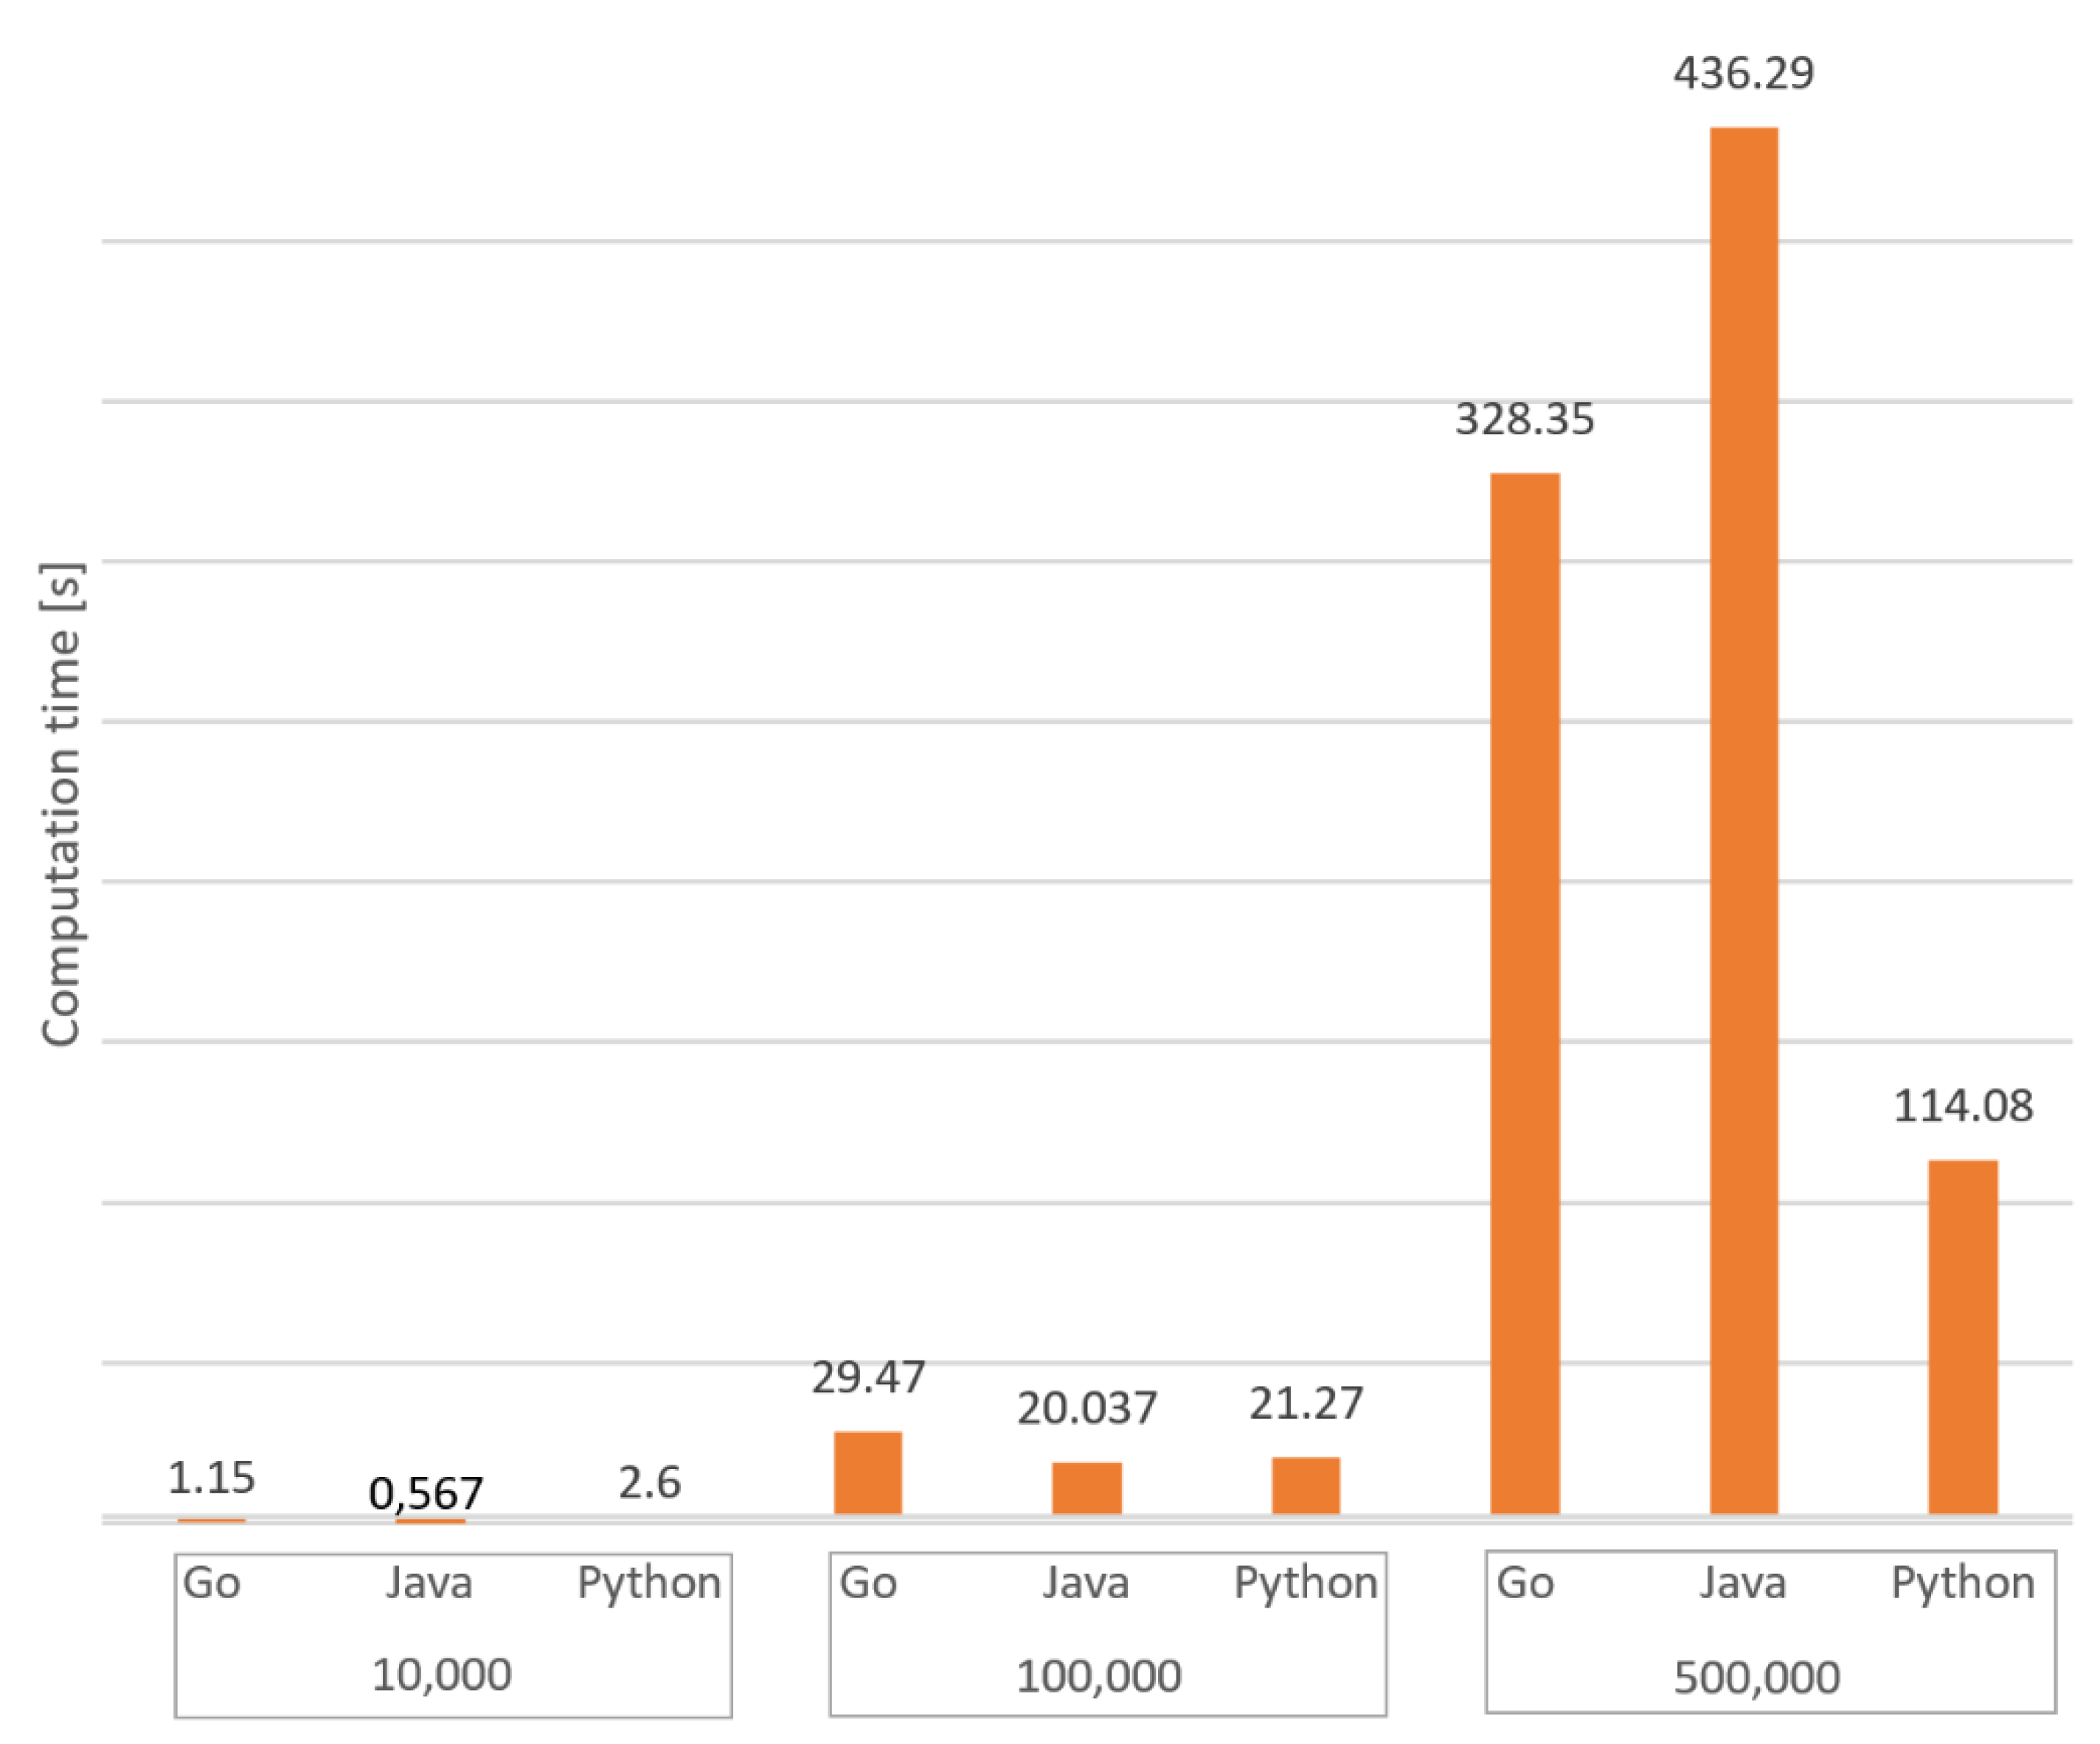
\includegraphics[height=0.3\textheight]{./part/Proyecto_ejecutivo/memoria_constructiva/golang/img/compTime}
	\caption[performance golang on algorithm]{performance golang on algorithm\cite{Dymora20201}}\label{fig:performance golang}
\end{figure}

El verdadero motivo para optar por golang como lenguaje viene más de la mano de la facilidad de mantenimiendo, la rapidez de compilacion, el manejo fácil para la concurrencia y eficiente en el uso de recursos. Implementar mecanismos de memoria compartida para procesos concurrente es donde golang si optimiza recursos. Uno de los trabajadores de google que ha contribuido al ecosistema de Golang nos dice “Everyone knows and thinks about Google in terms of scale of users and scale of servers, but one thing that's not talked about as often is the scale of engineering effort.“~\cite{Meyerson2014104+101}. Esto quiere decir que en la mayoría de las compañías el mayor coste no es el de infraestructura, si no el de ingeniería. Es un factor más importante el reducir el numero de horas dedicadas a mantener y desarrollar software que el hecho de optimizar el uso de máquinas. Si encima nos encontramos con un problema que no requiere de uso intensivo en cuestión algorítmica o tiempo de respuesta encontramos lo mejor de los dos: tenemos la ventaja de reducir los recuros necesarios de infraestructura y los de ingeniería. Si se diera el caso de que el software se enfrenta con el tiempo a problemas de escala siempre nos quedará la opción de aumentar las prestaciones de las máquinas utilizadas pero no tener problemas de aumento de costes de ingeniería. El tiempo de compilación mientras se desarrolla un software puede llegar al orden de minutos por prueba en lenguajes como Java. Este coste elevando al orden de magnitud de una empresa como Google puede significar una ingente cantidad de horas.

Las referencias consultas aplicados a distintos casos de uso extraen las mismas conclusiones acerca del nicho de uso de Golang y las bondades y puntos débiles del mismo:

\begin{itemize}
	\item uso para blockchain~\cite{Ray202110857} o smartcontracts~\cite{Ding2021321}
	\item librerias para la depuración de códigos concurrentes~\cite{Taheri2021138}
	\item machine learning para reconocimientos de lenguajes~\cite{NoAuthor2021179,Dilley2019377}
	\item uso para IoT ~\cite{Samaniego2017116}
	\item análisis de flujos de carga en sistemas electricos, haciendo uso de la concurrencia para resolver con mayor rapidez el cálculo~\cite{Khaitan20152909}
	\item y otros usos varios de la paralelización de problemas~\cite{Qiu2018,Shoumik20181,Mladenovic2018,Benedict2017437,Irawan2017,Leokhin2015656,Komendantskaya2014121,Mittal2014292}.
\end{itemize}

Como conclusión citamos los resultados de~\cite{WhiteheadII2011209}“Despite the relatively young age of the programming language, we believe that Go helps to fill an interesting niche in the field of programming languages. The unique feature-set and aims of the language make it worth investigation for systems-level concurrent programming.“ Habiendo madurado el lenguaje unos años desde la publicación de este artículo encontramos que sigue siendo interesante y está altamente valorado en la comunidad de desarrollo de software. Nos permiten concluir que está justificado nuestro objetivo de diseñar un sistema de las caracteristicas de este proyecto con Golang.

